\documentclass[spanish,12pt]{elsarticle}
\usepackage{graphicx}
\usepackage{amssymb}
\usepackage{amsmath}
\usepackage{siunitx}
\usepackage{lineno}
\usepackage{babel}

\makeatletter
\def\ps@pprintTitle{%
  \let\@oddhead\@empty
  \let\@evenhead\@empty
  \let\@oddfoot\@empty
  \let\@evenfoot\@oddfoot
}
\makeatother

\abstracttitle{Resumen}

\begin{document}

\begin{frontmatter}
\title{Problema K-minimum spanning tree}
\author{Roberto Juan Cayro Cuadros, Gabriel Alexander Valdivia Medina,
Giulia Alexa Naval Fernández, Rodrigo Alonso Torres Sotomayor}
\begin{abstract}
    
\end{abstract}
\address{Universidad Católica San Pablo}

\end{frontmatter}

%%
%% Start line numbering here if you want
%%

%% main text
\section{Introducción al problema}
El k-MST o k-minnimum spanning tree problem, árbol de expansión de péso mínimo k en español es un problema computacional que pide un árbol de mínimo costo con exactamente $k$ vértices que forme un subgrafo del grafo original. \cite{1}\\%wikipedia
\begin{figure}[h]
    \centering
    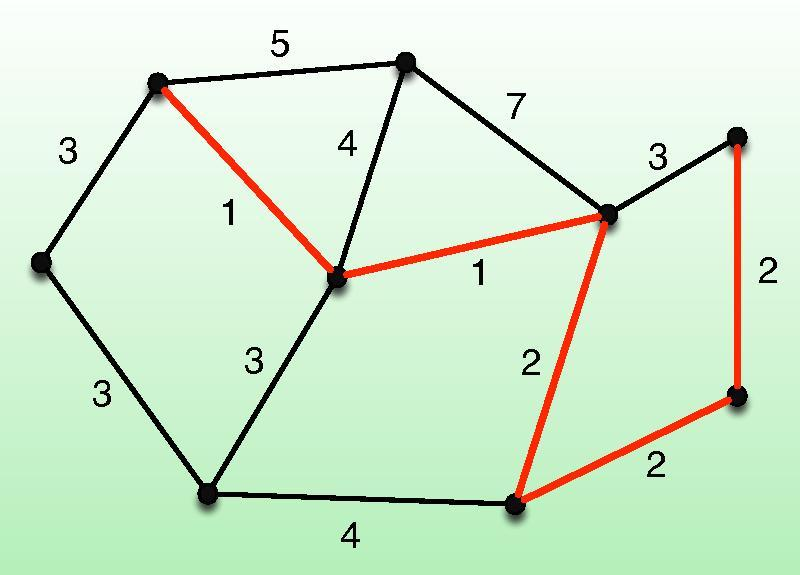
\includegraphics[scale=0.5]{images/6-mst.jpg}
    \caption{6-MST del grafo G. Fuente: Wikipedia Commons}
    \label{fig:my_label}
\end{figure}
%---------------------------------------------------------%


\section{Demostración NP-completo}
\paragraph{\textnormal{No es posible suponer la naturaleza del problema, y establecer que es NP-hard o NP-completo, sin la evidencia correspondiente, para probrarlo este debe pertenecer a NP, ademas que un problema NP-completo pueda reducirse al mismo}}
\subsection{Demostrar que k-MST $\in$ NP}


\subsection{Transformación NP-completo $\alpha$  k-MST}
\subsubsection{Steiner problem}
Es un problema NP-completo de los 21 problemas de Karp, usado en problemas de optimización y mayormente enfocado en estructuras de grafos aunque tambien visto en aplicaciones de modelación de redes con más de 2 terminales. El problema consiste en que,  dado un grafo no-dirigido de aristas con peso, generar un arbol dado un
\textit{Sub-set} de vertices los cuales formarán este arbol. Además, pueden añadirse nuevos vertices para lograr las conexiones entre estos, llamados \textit{Steiner-vertices}.\\\\
El objetivo del problema será crear un arbol de menor peso posible, tomando en cuenta los pesos, y los vertices dados. Los vertices deberán ser exactamente los dados en el Sub-set, pero podrán ser añadidos los Steiner-vertices fueran necesarios.
La principal diferencia con el k-MST es que aquí recibimos un conjunto específico de vectores para conformar nuestro árbol, pudiendo usar vértices fuera de la relación para conectarlos. El k-MST no recibe esta relación, sólo el número de vértices exactos que necesita.\\ 


\subsection{Transformación}
\subsubsection*{Steiner-problem}
\textit{Entrada: }
\begin{itemize}
\item Grafo no-dirigido G con aristas de peso.
\item Sub-set de vertices S.
\end{itemize}

\textit{Salida: }
\begin{itemize}
\item Arbol de menor peso con los vertices de S y los Steiner-vertices si fueran necesarios.\\
\end{itemize}
\clearpage
\subsubsection*{k-MST}
\textit{Entrada: }
\begin{itemize}
\item Grafo no-dirigido G con aristas de peso.
\item Número k
\end{itemize}

\textit{Salida: }
\begin{itemize}
\item Arbol de menor peso con k-vertices y k-1 aristas.
\end{itemize}

\subsubsection{Reducción}
\textnormal{Dada la entrada G para Steiner, se puede tomar el mismo grafo para k-MST, puesto que tiene las aristas pesadas y un número determinado de vertices. Aún debe aplicarse una transformación polinomial, de modo que usaremos su complemento cuyas aristas serán de peso igual a size of sub-set, de esta forma aseguramos la transformación y no afectara la salida porque siempre busaremos el arbol de menor peso , se usará el tamaño del sub-set de vertices siendo este igual a k.}\\\\
\textnormal{Por consiguiente logramos reducir el problema de Steiner tree a k-mst, al tranformar su entrada en los parámetros de k-MST. Pero resta confirmar que la solución de k-MST también podría solucionar a Steiner-tree. La salida de k-mst será un arbol con el menor peso posible, sin embargo, debemos tener en cuenta que el número k denota la cantidad de vertices necesarios más no que vertices, por lo tanto el numero total de permutaciones de los vertices de G serán combinaciones de el número total de vertices(n) en k vertices:}\\\\
\textit{
\[
\textnormal{Total~de~permutaciones (Tn)}= \binom{n}{k} = \frac{n!}{k!(n - k)! }.
\]
}
\textnormal{Esto es importante porque sabiendo que k es el size of sub-set (S) , y hablamos de todas las permutaciones de ese tamaño, podemos concluir que el S debe estar incluido en Tn. Por ello:  }\\\\
\textit{
\[
S \subseteq Tn
\]
}\\\\
Sin embargo, calcular todas las permutaciones de una cantidad $n$ de elementos es un proceso con una complejidad $O(!n)$, que no entra dentro de complejidad polinomial. Es necesario otro tratamiento para que el k-MST opere con los vértices que el algoritmo Steiner pide. Otra idea es añadir un árbol con aristas de peso 0 en cada vértice que pertenezca a la relación de vértices de Steiner. De esta forma, el k-MST utilizará estos vértices sí o sí como parte de su solución.
Calculamos $t$ (número de vértices en cada uno de estos árboles de arista 0) como $t = n-r-1$, siendo n el número de vértices totales y r el tamaño del sub-set de Steiner.\\\\ 
\begin{figure}[h]
    \centering
    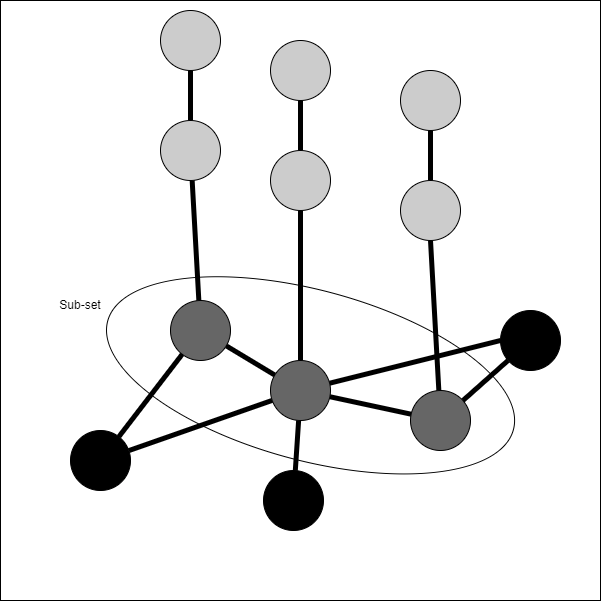
\includegraphics[scale=0.5]{images/Trans_graph.png}
    \caption{Transformación de la entrada de Steiner a entrda de k-MST. Elaboración propia.}
    \label{fig:my_label}
\end{figure}
\section{Algoritmo de fuerza bruta}
\section{Algoritmo aproximado}


%% References
%%
%% Following citation commands can be used in the body text:
%% Usage of \cite is as follows:
%%   \cite{key}          ==>>  [#]
%%   \cite[chap. 2]{key} ==>>  [#, chap. 2]
%%   \citet{key}         ==>>  Author [#]

%% References with bibTeX database:

\bibliographystyle{model1-num-names}
\appendix
\section*{Bibliography}
\bibliography{sample.bib}

%% Authors are advised to submit their bibtex database files. They are
%% requested to list a bibtex style file in the manuscript if they do
%% not want to use model1-num-names.bst.

%% References without bibTeX database:

\begin{thebibliography}{00}
\bibitem{1} 
https://en.wikipedia.org/wiki/K-minimum\_spanning\_tree
%% \bibitem must have the following form:
%%   \bibitem{key}...
%%

% \bibitem{}

\end{thebibliography}
%https://en.wikipedia.org/wiki/K-minimum_spanning_tree
%https://www.geeksforgeeks.org/steiner-tree/
%https://pages.cs.wisc.edu/~shuchi/courses/880-S07/scribe-notes/lecture26-2.pdf

\end{document}

%%
%% End of file `elsarticle-template-1-num.tex'.
